% Chapter 1

\chapter{Project Design} % Main chapter title

\label{Chapter3} % For referencing the chapter elsewhere, use \ref{Chapter1}

\lhead{Chapter 3. \emph{Project Design}} % This is for the header on each page - perhaps a shortened title

%----------------------------------------------------------------------------------------

\section{Methodology}
The methodology adopted for designing the "Track A Shop: Web App" is an iterative process. The methodology encompasses various stages from project initiation to implementation, ensuring an organized and systematic approach as each stage is mentioned below:

\begin{figure}[h]
	\centering
	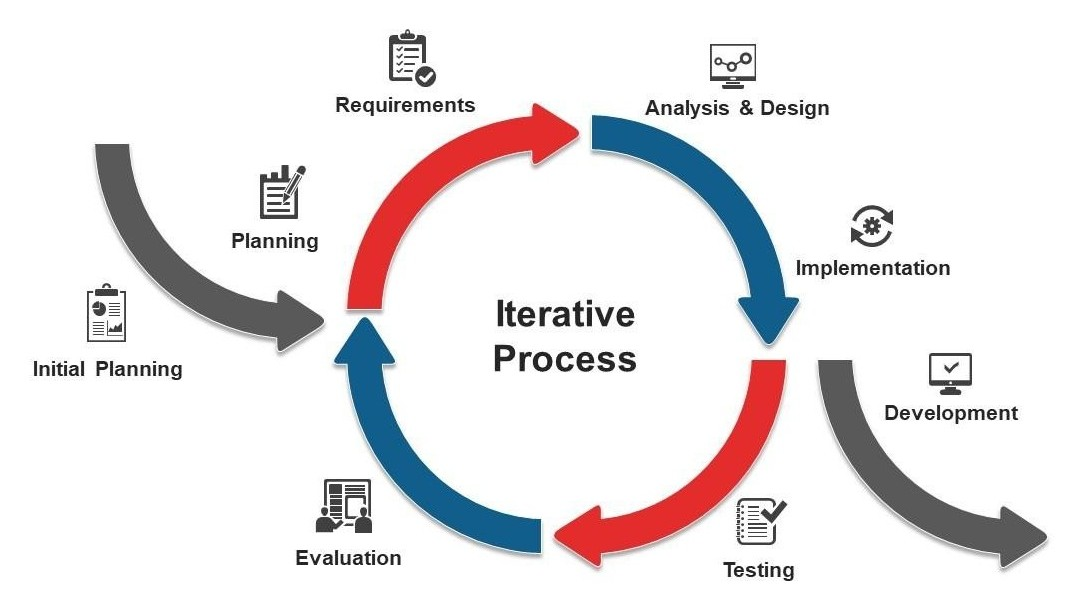
\includegraphics[width=15cm]{iterative_process_model}
	\caption{Iterative Process Model}
\end{figure}

\subsection{Initial Planning}

In this initial planning stage, the project goals and initial requirements are outlined. Key activities include:

\textbf{Defining Project Goals}: Setting the overall goals and vision for the "Track A Shop: Web App".

\textbf{Preliminary Requirement Analysis}:
Performing an initial analysis of high-level requirements and constraints.

\subsection{Planning}

The planning stage involves planning the upcoming iteration and setting specific goals for it. Key activities include:

\textbf{Setting Iteration Goals}:
Defining the objectives and outcomes for the current iteration.

\textbf{Identifying Resources}:
Allocating the necessary resources, including manpower, technology, and tools, for the iteration.

\subsection{Requirements Analysis and Design}

In this stage, detailed requirements are gathered and analyzed, and the system's design is conceptualized. Key activities include:

\textbf{Requirements Refinement}:
Analyzing and refining requirements based on feedback from previous iterations and stakeholders.

\textbf{System Design}:
Conceptualizing the system's design and architecture based on the refined requirements.

\subsection{Implementation and Development}

The implementation stage involves writing code and developing the iteration. Key activities include:

\textbf{Coding and Development}:
Writing the code based on the design and architecture defined in the previous stage.

\textbf{Integration}:
Integrating the developed components and modules into a cohesive iteration.

\subsection{Testing}

The testing stage involves validating the functionality and performance of the developed iteration. Key activities include:

\textbf{Functional Testing:}
Ensuring that the iteration meets the specified functional requirements.

\textbf{User Acceptance Testing:}
Engaging users to validate the iteration against their expectations and requirements.

\subsection{Evaluation}

The evaluation stage involves assessing the outcomes of the iteration. Key activities include:

\textbf{Evaluation of Goals}:
Evaluating whether the iteration goals were achieved and identifying areas for improvement.

\pagebreak

\subsection{Development Stage}

The development stage of the "Track A Shop: Web App" project involves translating the project design and requirements into functional software components. This stage is characterized by a series of iterative cycles, each aimed at enhancing and expanding the platform's features.

\begin{enumerate}
	\item \textbf{Iteration 1: Initial Prototyping}
	
	The first iteration focuses on creating a basic prototype of the web application, emphasizing core features such as user registration, product listing, and basic geolocation functionalities. User feedback is collected to inform further development.
	
	\item \textbf{Iteration 2: Image Recognition Integration}
	
	Building upon the initial prototype, the second iteration introduces image recognition technology to simplify product and service listing. Sellers can now capture or upload images, and the system automatically populates product/service details.
	
	\item \textbf{Iteration 3: Geolocation and User Interface}
	
	This iteration enhances geolocation features, allowing customers to search for nearby shops and products/services within a specified radius. Simultaneously, the user interface is refined, focusing on aesthetics and usability.
	
	\item \textbf{Iteration 4: User Feedback and Usability}
	
	The fourth iteration revolves around collecting user feedback and making usability improvements. User testing and feedback surveys are conducted to identify pain points and areas for enhancement.
	
	\item \textbf{Iteration 5: Scalability and Performance}
	
	With a more refined platform, the fifth iteration addresses scalability and performance optimization. Measures such as caching, load balancing, and database query enhancements are implemented.
	
	\item \textbf{Iteration 6: Integration and Security}
	
	In this phase, third-party integrations, enhanced security measures, and multi-language support are introduced. Payment gateways are integrated to facilitate seamless transactions.
	
	\item \textbf{Iteration 7: Testing and Quality Assurance}
	
	The final iteration focuses on comprehensive testing and quality assurance. Unit testing, integration testing, and user acceptance testing are conducted to ensure the platform's reliability and performance.
\end{enumerate}

The iterative development approach ensures that each phase builds upon the previous one, allowing for continuous improvements and a more robust final product.


\newpage

\section{Architecture Overview}


\begin{figure}[h]
	\subsection{Class Diagram (UML) }
	\centering
	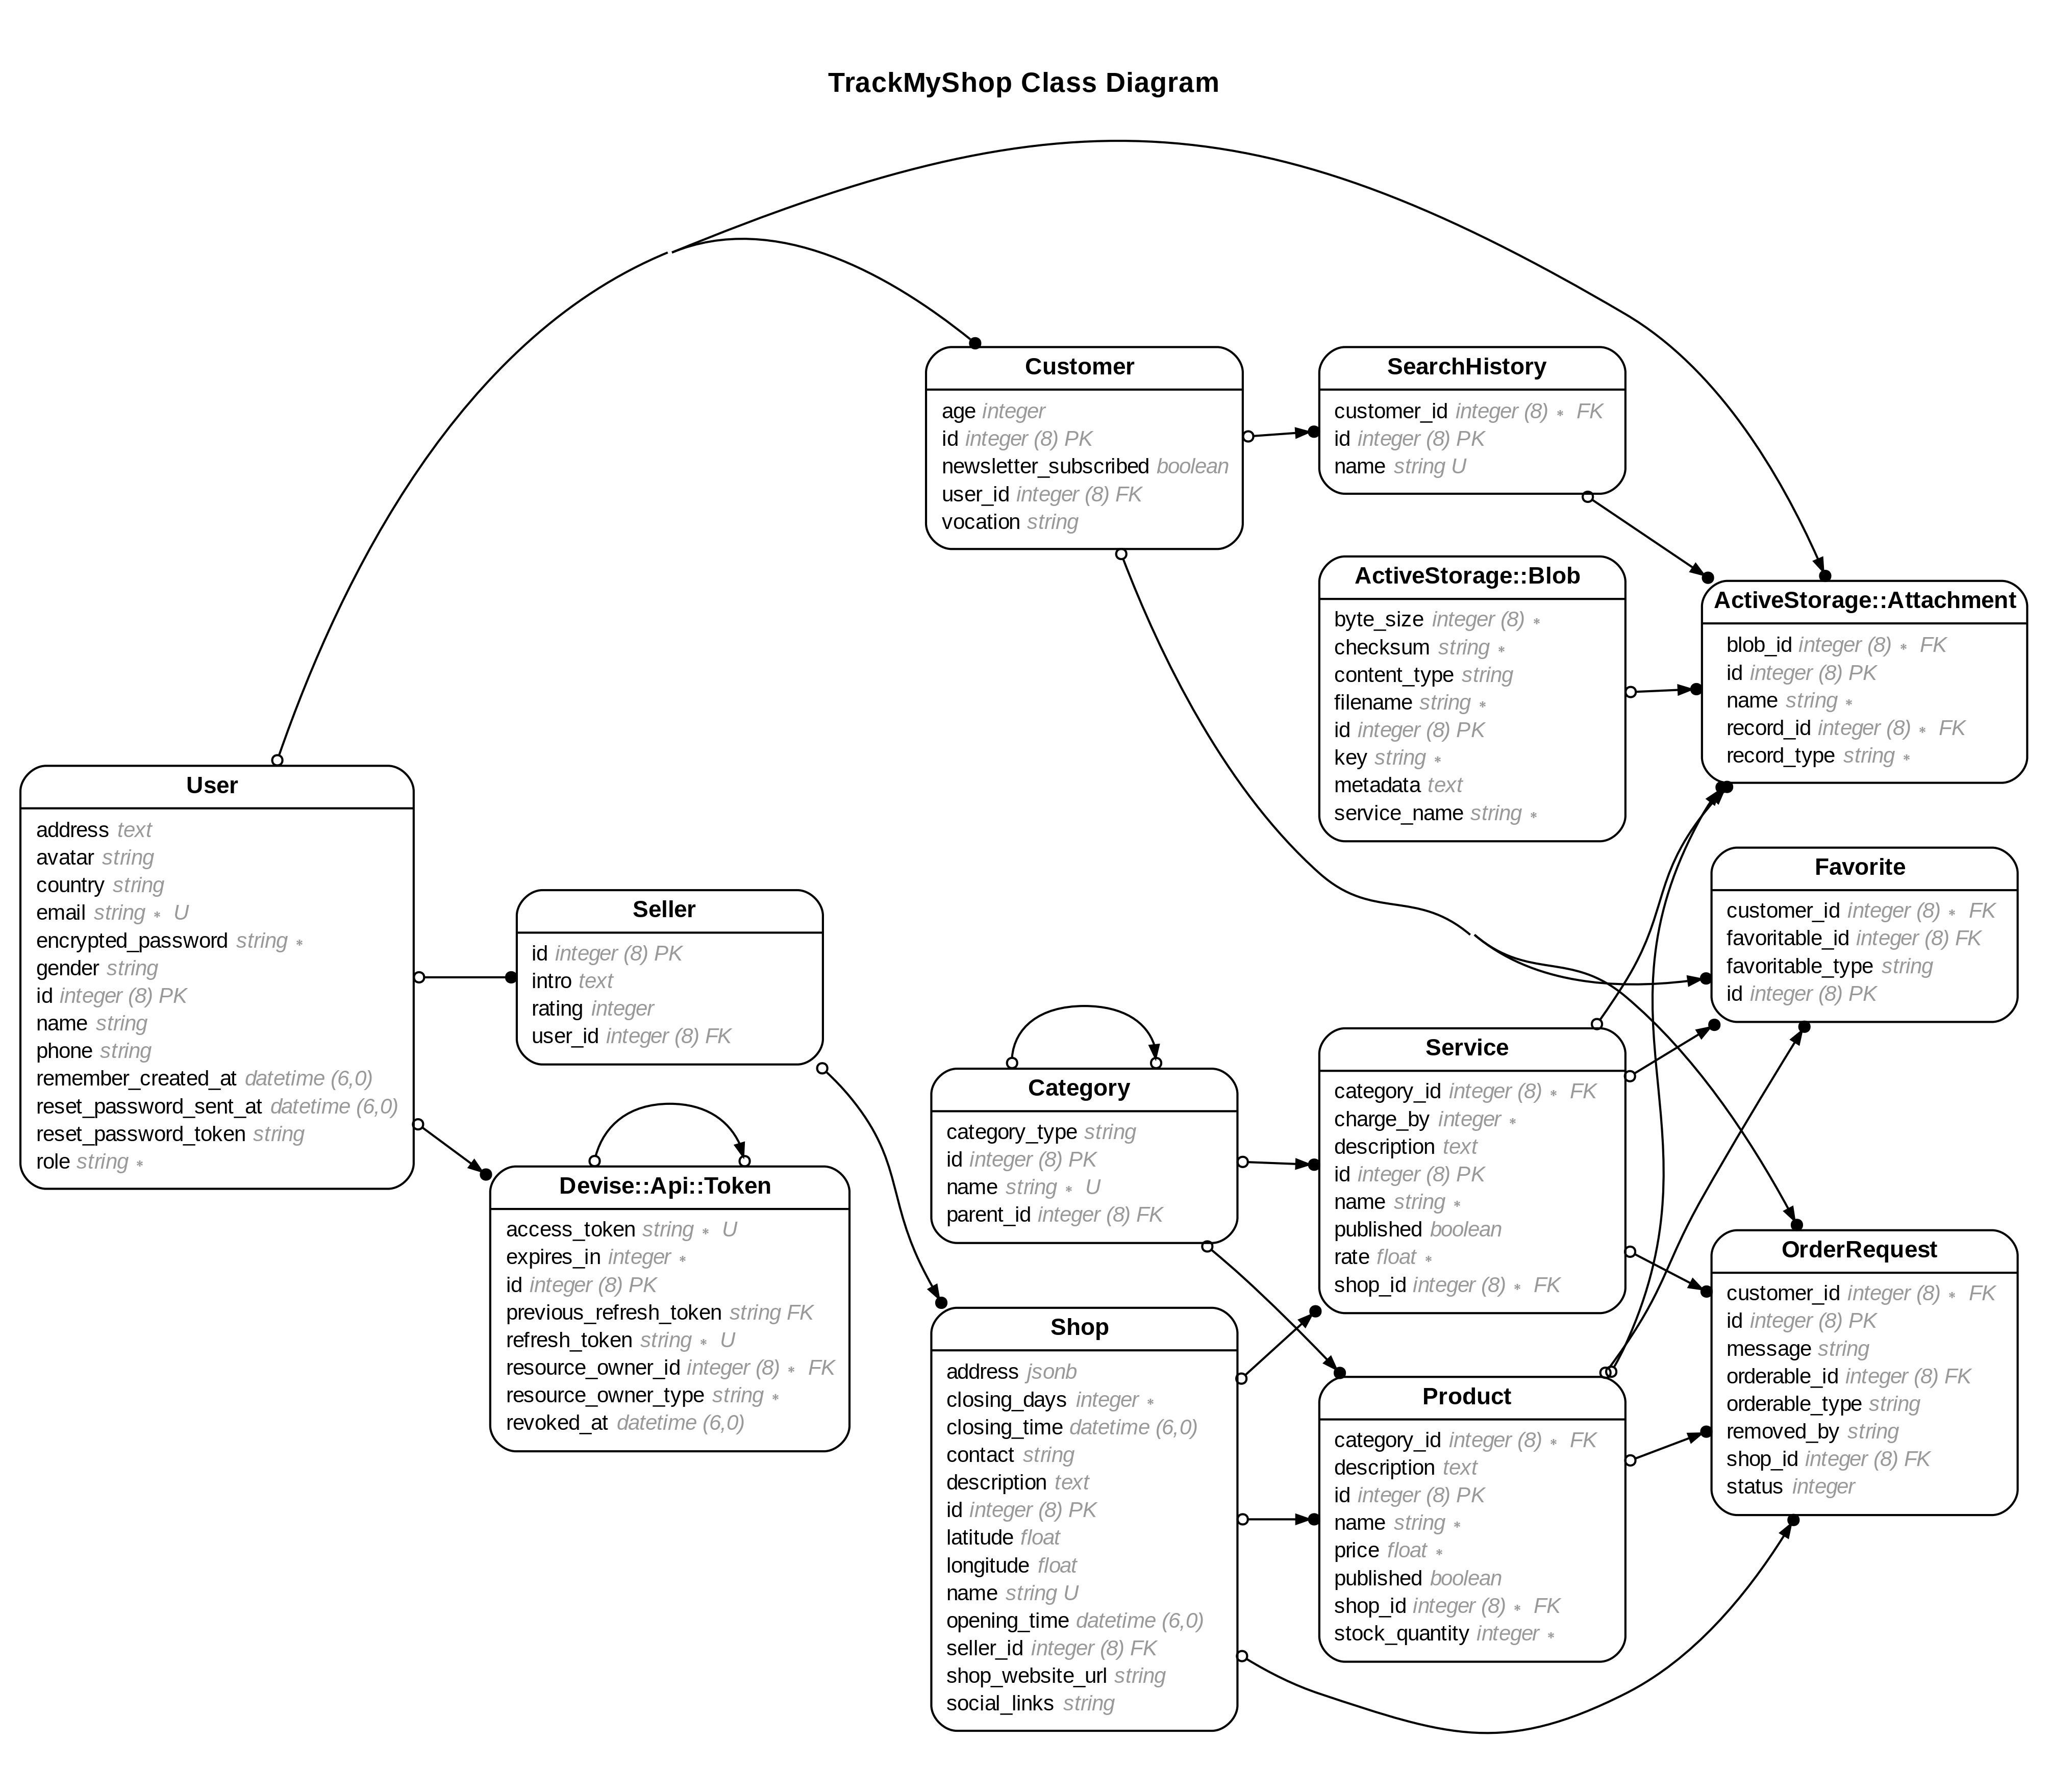
\includegraphics[width=17cm]{TrackMyShop_CD}
	\caption{Track A Shop: Web App - Class Diagram}
\end{figure}

\pagebreak
\begin{figure}[h]
	\subsection{Customer Sequence Diagram \\\\}
	\centering
	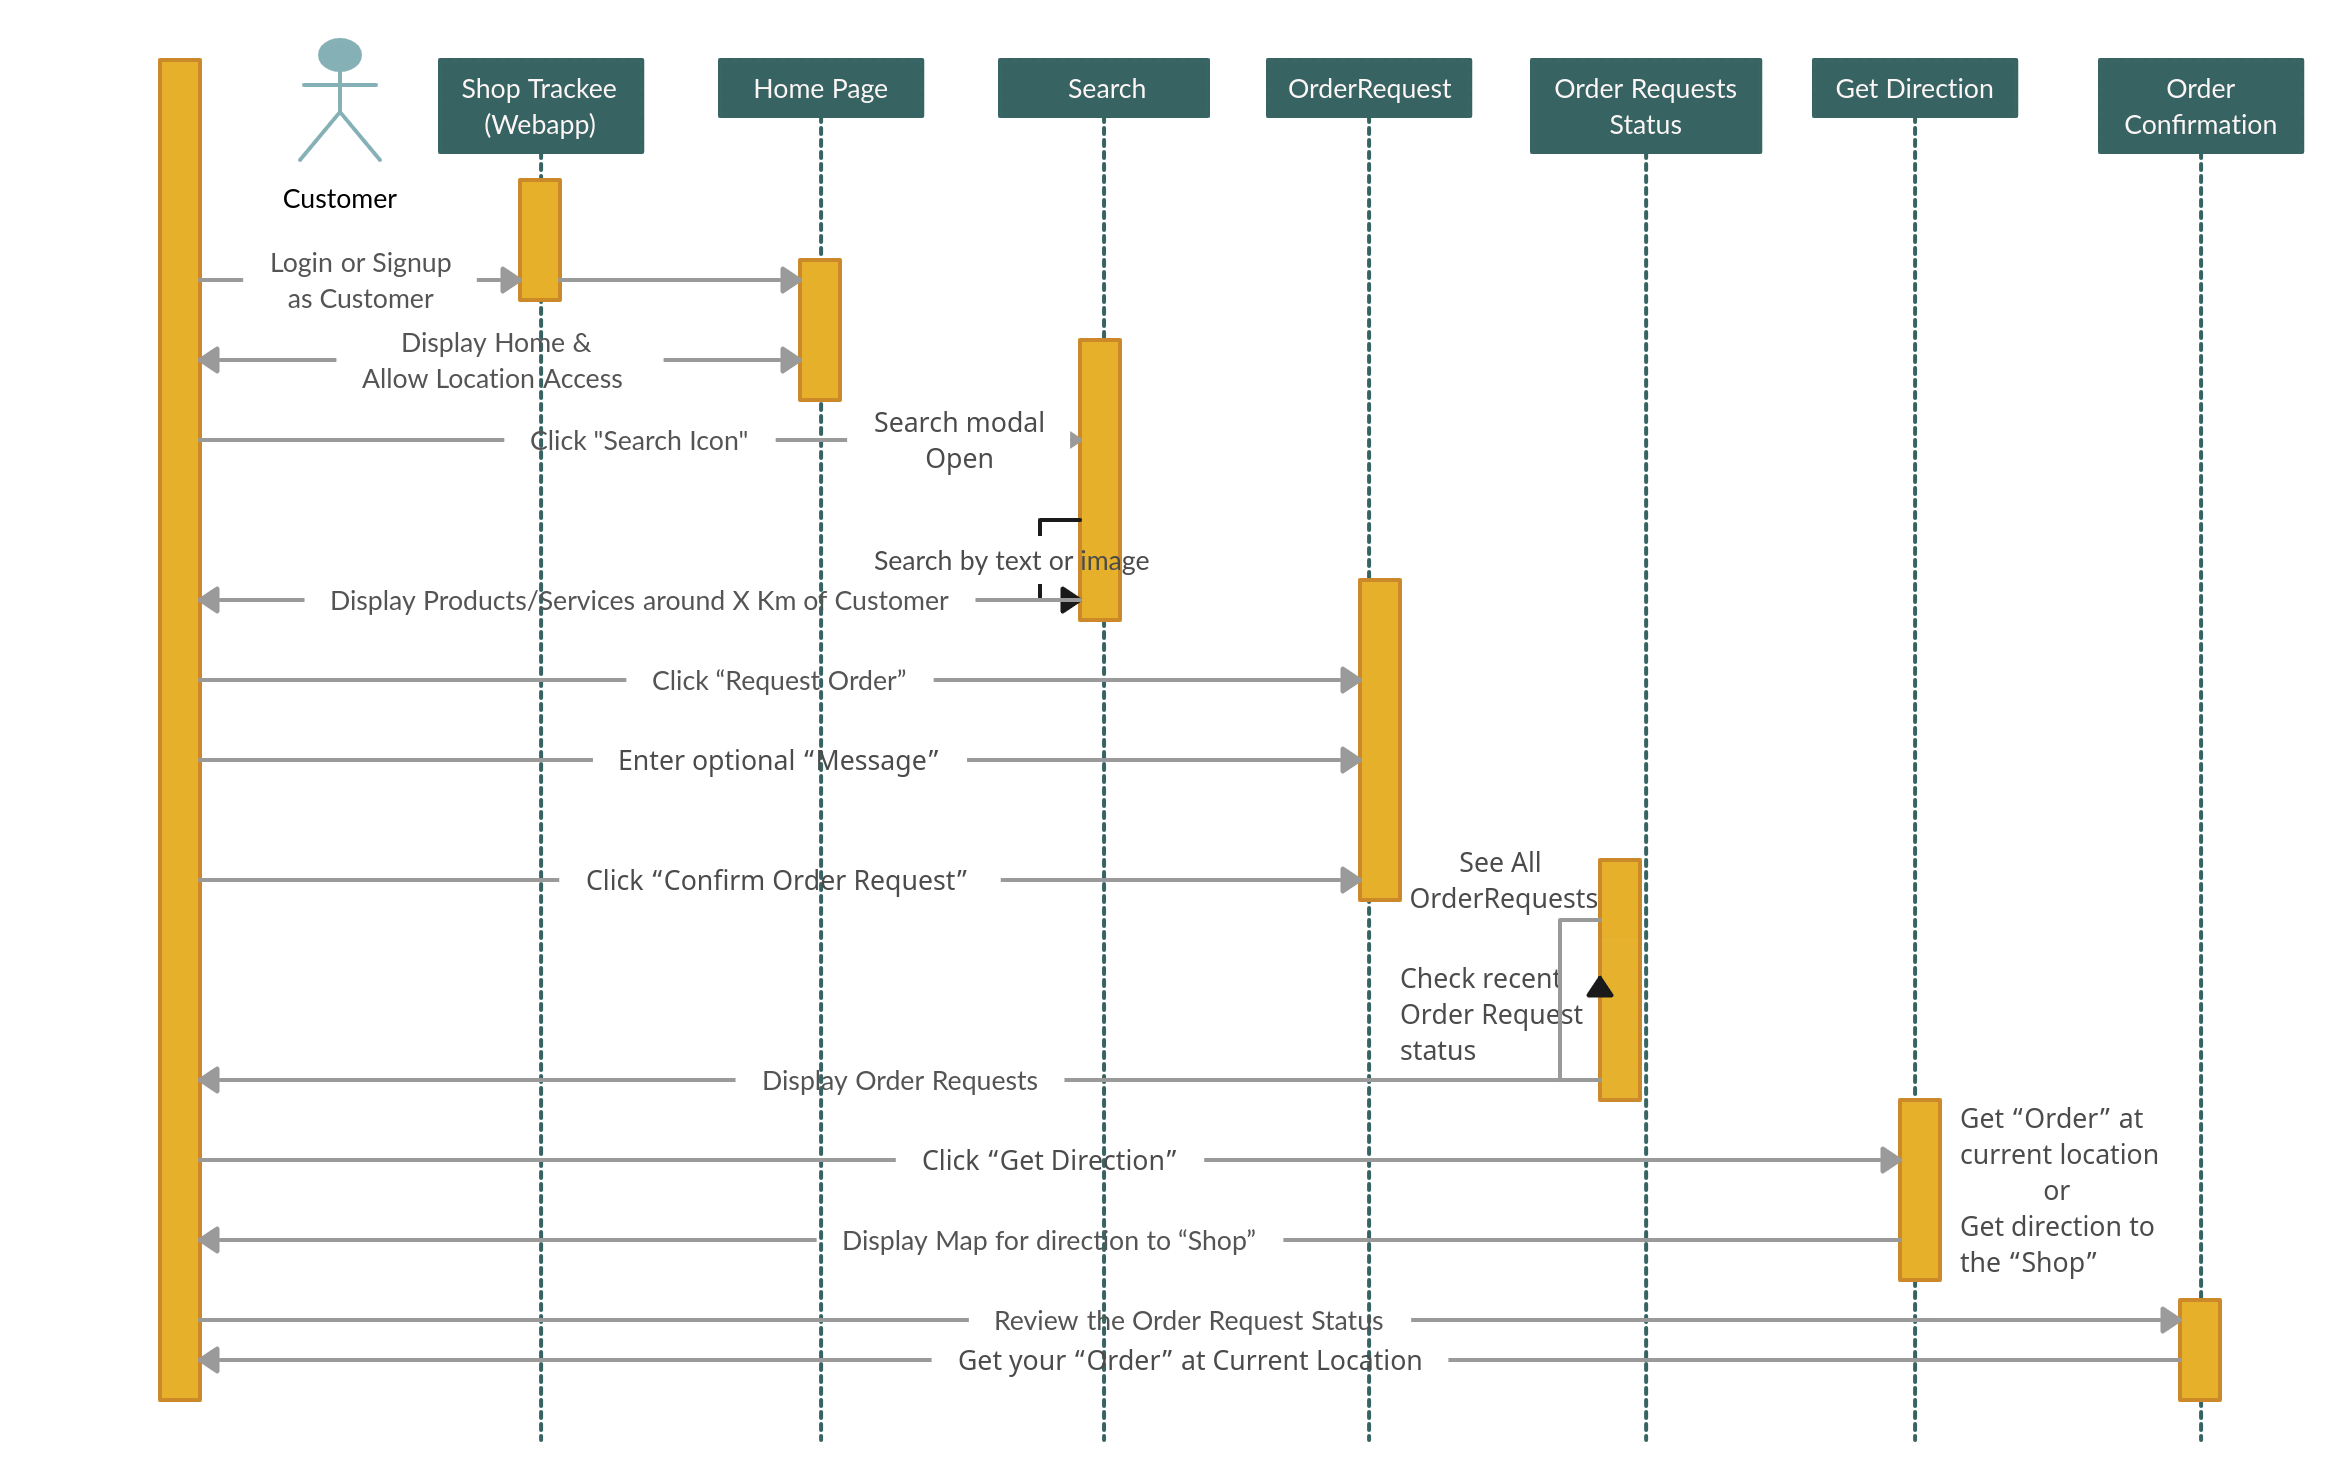
\includegraphics[width=1.1\linewidth]{customer-sequencedigram}
	\caption{Track A Shop: Web App - Customer Sequence Diagram}
\end{figure}

\pagebreak
\begin{figure}[h]
	\subsection{Seller Sequence Diagram \\\\}
	\centering
	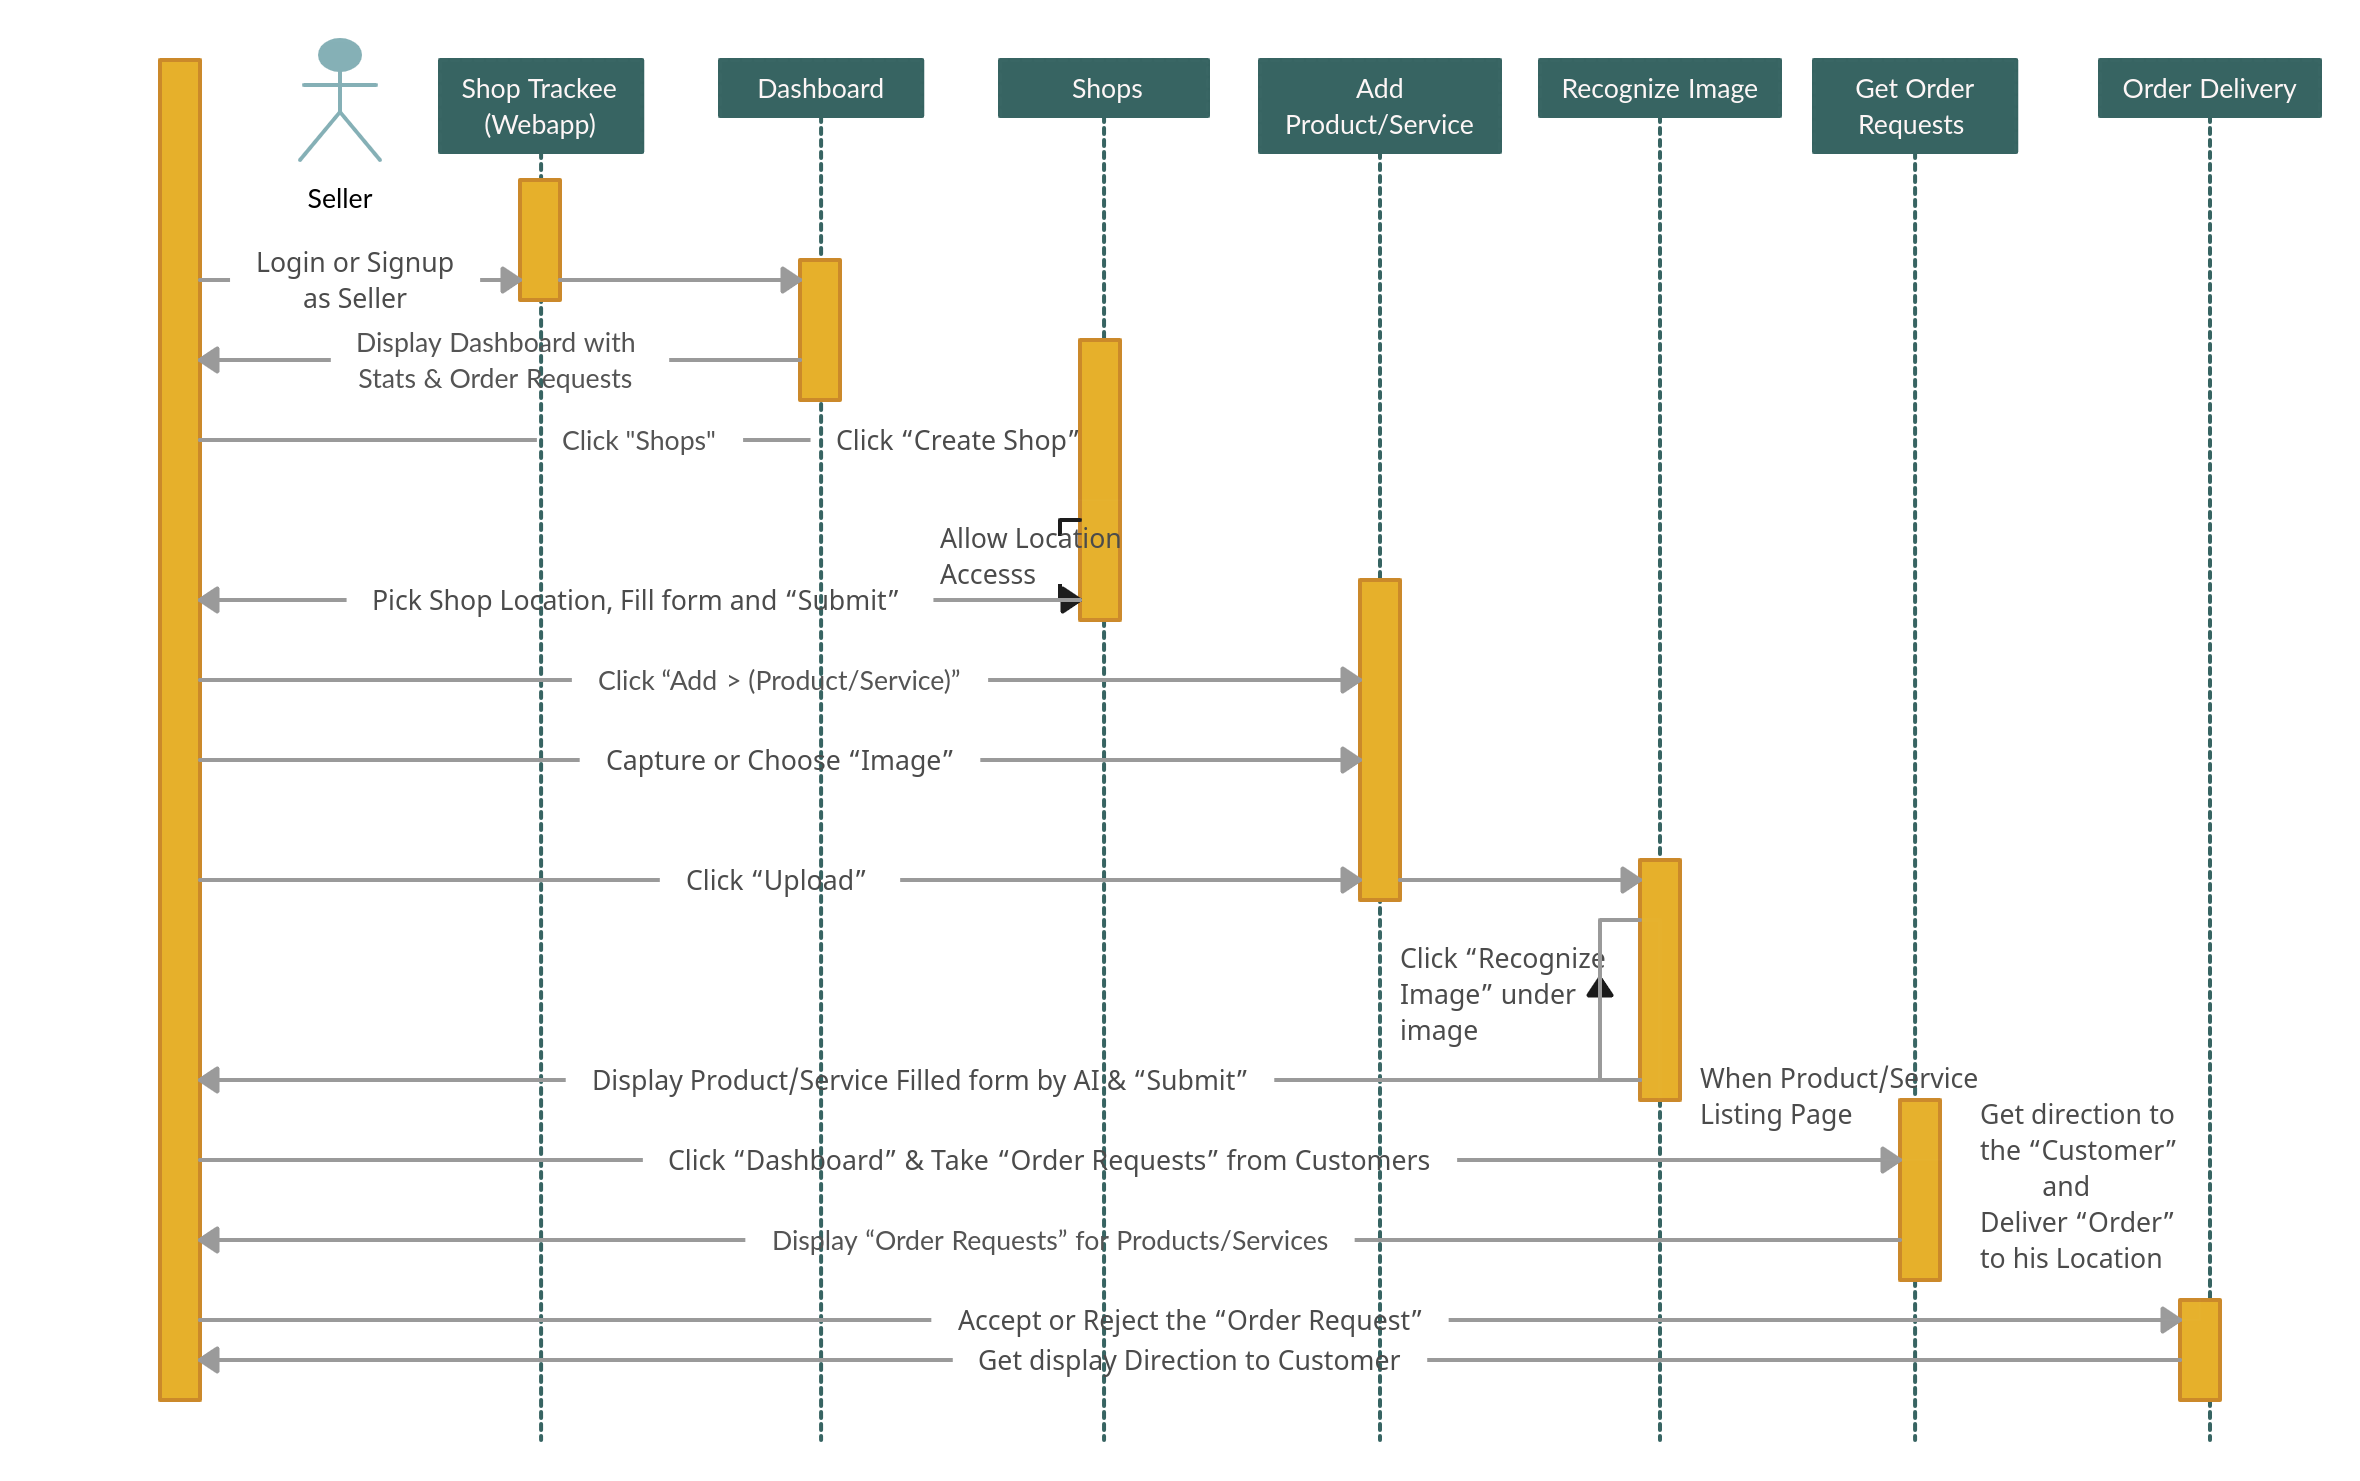
\includegraphics[width=1.1\linewidth]{seller-sequence-diagram}
	\caption{Track A Shop: Web App - Seller Sequence Diagram}
\end{figure}


\pagebreak

\begin{figure}[h]
	\section{Design Description}
	Here is the basic architectural design of our Web Application:\\
	\vspace{1.5cm}
	\centering
	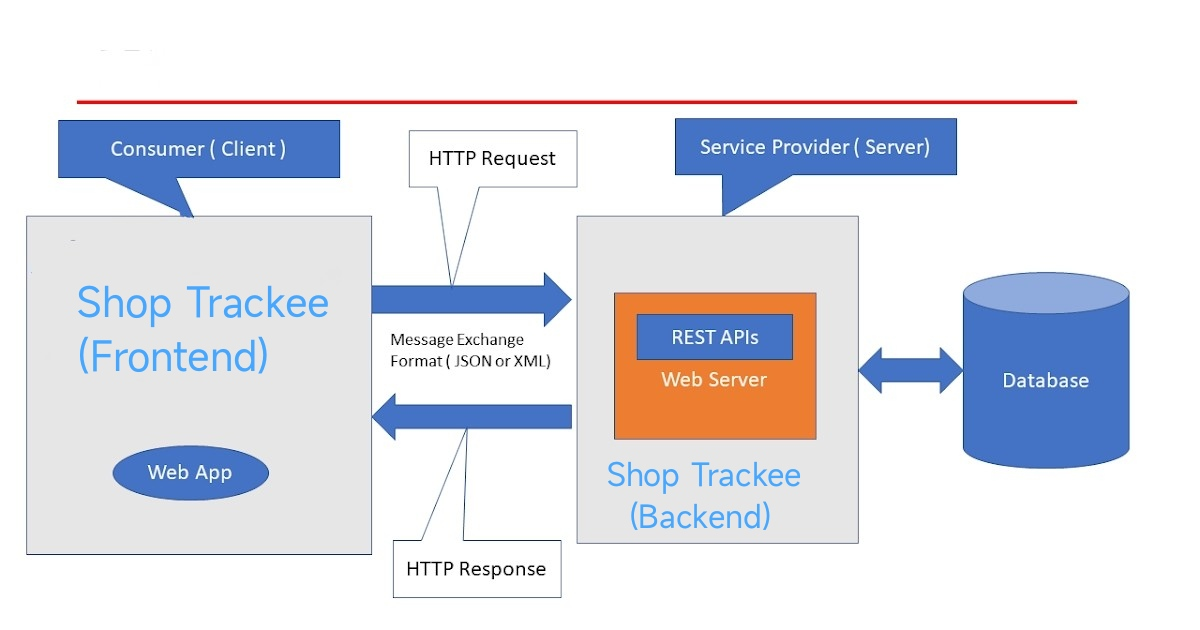
\includegraphics[width=1\linewidth]{design-description}
	\caption{Track A Shop: Web App - Design Description}
\end{figure}
\pagebreak


